\section{Introduction and the mathematical synthesis problem}\label{sec:intro}
\subsection{The problem}
Fix the two maps
\[
T_N(m)=m\frac{(N+1)^2}{N}\quad(N\mid m,\ m,N\in\Z_{\ge1}),\qquad C(x)=x+\frac{L(x)^2}{G(x)}\quad(x\in\Q_{>0}),
\]
where, for $x=a/b$ in lowest terms, $D(x)=\{d\ge2:\ d^2\mid a,\ d\equiv1\pmod b\}$, $L=\lcm D(x)$ and $G=\gcd\{d-1:d\in D(x)\}$. The first map composes into \emph{histories} $(m_0;N_1,\dots,N_r)$ that reach an integer; the second is a deterministic dynamics. Both maps are governed by divisibility of a numerator by squares, and both attach to their states the same kind of object: an occurrence set $D$, an arithmetic lattice of relations among the occurrences, a set of primitive relations in it, and cell complexes built from them. The three technical manuscripts of this programme studied these objects separately: lattice transport and its dimensional obstructions~\cite{PaperI}, the topology of the spaces of histories~\cite{PaperII}, and the evolution of the complexes along collective orbits~\cite{PaperIII}. The present manuscript asks a single question.

\begin{quote}\emph{Which of these structures determine which others, and where exactly do the determinations fail?}
\end{quote}

An answer has a definite logical form. A determination is a \emph{factorization}: a map $f$ factors through a map $\pi$ exactly when $f$ is constant on the fibres of $\pi$ (\cref{lem:factor}). A failure of determination is an \emph{obstruction}: two points of the domain with the same image under $\pi$ and different images under $f$. Every claim below is of one of these two forms, or is an explicitly marked open construction, or is an interpretive comparison without a claimed correspondence.

\paragraph{What the synthesis says about the Substrate.} The mathematical question has a structural counterpart: what do these results say about the generative architecture of the UNNS Substrate itself? The answer given here is deliberately operational. States, histories, occurrence inventories, primitive relations and realised complexes are linked by the proved factorizations, admissibility conditions and obstructions of \cref{sec:diagram,sec:register}, and \cref{sec:characterisation} states what these relations support and what they do not. It is a synthesis conclusion, not a numbered theorem.

\subsection{The four governing questions}
We retain the four organising questions of the programme and answer each by a proposition, an obstruction, a conditional result or a precise open problem.
\begin{description}[leftmargin=1.2em,itemsep=2pt]
\item[S1 (common guards).] The admissibility condition $N\mid m$ of a history step and the occurrence condition $d^2\mid a$, $d\equiv1\ (b)$ of a collective event both involve divisibility of the integer by squares and congruences. For integer states the two guards coincide exactly (\cref{prop:P2}(a), a bijection between occurrences and incoming steps); for rational states the congruence $d\equiv1\ (b)$ has no counterpart in the generative rule, and a rational extension is an open construction (\cref{sec:open}, O8).
\item[S2 (information lost by projection).] The chain endpoint $\leftarrow$ content $\leftarrow$ swap class $\leftarrow$ history, and the chain $x\mapsto D(x)\mapsto$ realised complex, are chains of factorizations; every step loses information, with exact witnesses (\cref{prop:P1,prop:P2,prop:P5}). The data that \emph{do} reconstruct a history are the occurrence sets along the whole path (\cref{thm:faith-cited}), not the occurrence set of the endpoint.
\item[S3 (geometry across spaces).] The complex of an integer state is determined by $D$; the history space of the same integer has independent arithmetic. The endpoint occurrence complex does not determine the associated history complex or its recombination invariants (\cref{prop:P5}); a general structure-preserving correspondence remains unestablished. Relations between history spaces and evolving complexes beyond the level of occurrence labels are open (\cref{prop:P9}, O3).
\item[S4 (boundaries and events).] The transport criterion of Paper~I and the edge-loss criterion of Paper~III are instances of one abstract monotone-minimality principle (\cref{lem:minimal,prop:P3}); a direct comparison of the two ambient orders is an open problem (O7).
\end{description}

\subsection{Contributions and what is not claimed}
The new mathematics of this manuscript consists of nine propositions \SIV{1}--\SIV{9} with independent proofs (\cref{sec:register} gives the register), five lemmas used in them (Appendix~\ref{app:proofs}), the global diagram (\cref{fig:global}), and exact witnesses recomputed from scratch (Appendix~\ref{app:finite}). Results of Papers~I--III are cited with their theorem numbers and crosswalk identifiers (Appendix~\ref{app:prov}); they are not proved again unless a new derivation needs them in a modified form. Computations quoted from those manuscripts keep their original status; the verification of the frozen releases is inherited and was not re-run.

We do \emph{not} claim a universal organising law, a general commuting diagram between the generative and collective sides (\cref{sec:diagram} shows that none of the natural squares is claimed to commute), or any result about the third constant-type conjecture of the programme (statement C3 remains unclaimed). Finite-exact statements are never extrapolated.

\subsection{Reading guide}
\cref{sec:objects} fixes definitions. \cref{sec:numerical,sec:occurrence} treat the two projections; \cref{sec:realization,sec:history,sec:endpoint} treat geometry, history topology and their separation; \cref{sec:evolution,sec:prediction,sec:recurrence} treat evolution; \cref{sec:correspondence} compares the two dynamics; \cref{sec:diagram} presents the global diagram; \cref{sec:register,sec:theories,sec:conclusions,sec:open} collect results, relations to known theory, conclusions and open problems. Arrow conventions in all diagrams: a black solid arrow is an \emph{established arrow}; a thick green arrow is a \emph{proved factorization}; a red arrow with a cross and a bar is a \emph{proved obstruction}; a grey dashed arrow is an \emph{open construction}; a purple dotted double-headed arrow is an \emph{interpretive comparison}.

\noindent\Cref{fig:arch} shows architecture of the programme.

\begin{figure}[t]\centering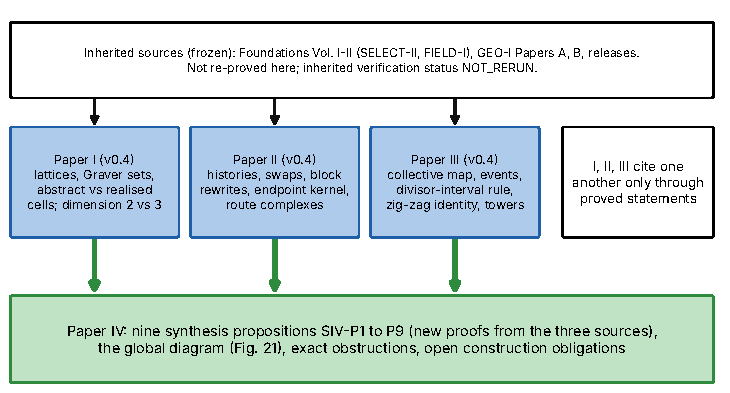
\includegraphics[width=\linewidth]{fig01_architecture.pdf}
\caption{\textbf{Architecture of the programme.} Paper~IV draws only on proved statements of Papers~I--III (v0.4) and on the frozen foundations. \emph{Schematic of inheritance; no mathematical object is drawn.}}\label{fig:arch}\end{figure}
